% plantilla de IEEEtrans (usada por el clei)
% #apt-get install texlive-publishers
\documentclass[conference]{IEEEtran}

% *** GRAPHICS RELATED PACKAGES ***
\usepackage{graphicx}
% declare the path(s) where your graphic files are
\graphicspath{{imagenes/}}
% and their extensions so you won't have to specify these with
% every instance of \includegraphics
\DeclareGraphicsExtensions{.png}

%para usar acentos del español en el código fuente
% #apt-get install texlive-lang-spanish
\usepackage[spanish]{babel}
\selectlanguage{spanish}
\usepackage[utf8]{inputenc}

% correct bad hyphenation here
%\hyphenation{op-tical net-works semi-conduc-tor}


\begin{document}

% can use linebreaks \\ within to get better formatting as desired
\title{
    Laboratorio Experimental de Tecnologías Computacionales: lecciones
    aprendidas luego de dos años de trabajo}

% author names and affiliations
\author{
    \IEEEauthorblockN{Aurelio Sanabria Rodríguez}
    \IEEEauthorblockA{
        Instituto Tecnológico de Costa Rica\\
        Sede Interuniversitaria de Alajuela\\
        Alajuea, Costa Rica\\
        ausanabria@itcr.ac.cr}

    \and
    \IEEEauthorblockN{Diego Munguía Molina}
    \IEEEauthorblockA{
        Instituto Tecnológico de Costa Rica\\
        Sede Interuniversitaria de Alajuela\\
        Alajuea, Costa Rica\\
        dmunguia@itcr.ac.cr}

    \and
    \IEEEauthorblockN{Jaime Gutiérrez Alfaro}
    \IEEEauthorblockA{
        Instituto Tecnológico de Costa Rica\\
        Sede Interuniversitaria de Alajuela\\
        Alajuela, Costa Rica\\
        jgutierrez@itcr.ac.cr}
}

% make the title area
\maketitle


\begin{abstract}

%\boldmath
Los estudiantes universitarios tienen, en los proyectos de investigación y
extensión, oportunidades para poner en práctica los conocimientos aprendidos en
un contexto real. La carrera de Ingeniería en Computación del Tecnológico de
Costa Rica se comenzó a impartir en la Sede Interuniversitaria de Alajuela en el
año 2012 y para el momento de su apertura no se contaba con espacios de este
tipo. A mediados del año 2013 se plantea la creación del Laboratorio
Experimental como un espacio en el cual se puede contar con equipos
computacionales de bajo costo y donde los estudiantes pudieran participar en
proyectos de investigación y extensión planteados por profesores de la carrera
de Ing. en Computación. Este artículo presenta las experiencias aprendidas del
proceso a los dos años de haber iniciado. 


\end{abstract}

% no keywords
Palabras clave — estudiantes de grado, tecnología de bajo costo, software libre
%%%%  Nota: revisar estas palabras claves



% For peer review papers, you can put extra information on the cover
% page as needed:
% \ifCLASSOPTIONpeerreview
% \begin{center} \bfseries EDICS Category: 3-BBND \end{center}
% \fi
%
% For peerreview papers, this IEEEtran command inserts a page break and
% creates the second title. It will be ignored for other modes.
\IEEEpeerreviewmaketitle



\section{Introducción}

A finales del 2011 el Consejo de Escuela de Ingeniería en Computación acordó
comenzar a impartir la carrera en la Sede Interuniversitaria de Alajuela (SIUA).
En el año 2012 se recibieron los primeros estudiantes y en adelante cada año se
admiten entre 40 y 80 nuevos alumnos. Si bien la Sede Interuniversitaria de
Alajuela comenzó a funcionar desde el año 2008 el Tecnológico de Costa Rica no
tenía ninguna carrera de grado en la Sede, por lo que la apertura de Ing. en
Computación significó una gran oportunidad para los estudiantes de la zona pero
a la vez evidenció la ausencia de posibilidades académicas, más allá de la
docencia, para los estudiantes empadronados en la sede. 

Los proyectos de investigación y extensión en los que se involucran estudiantes
de la carrera de Ingeniería en Computación les ayudan a desarrollar algunas
destrezas técnicas que no están incluidas formalmente en el plan de estudios,
por ejemplo: metodologías de investigación o procesos de construcción de
aplicaciones de software. Adicionalmente otras habilidades de las llamadas
"blandas" son fortalecidas cuando se involucran en este tipo de proyectos, en
particular el trabajo en equipo y la expresión oral y escrita. 

La idea de proveer un espacio académico para que se involucren los estudiantes
de la carrera de Ing. en Computación del Tecnológico de Costa Rica en la SIU fue
la razón principal por la que a mediados del 2013 se planteó la creación del
Laboratorio Experimental de Tecnologías Computacionales (LabExp). Se solicitó la
adquisición de equipo computacional de bajo costo y herramientas de trabajo al
TEC y un espacio físico de trabajo a la administración de la SIU. Formalmente el
Laboratorio se planteó como una actividad de investigación aprobada por el
Comité Técnico del Centro de Investigaciones en Computación (CIC). En la
propuesta se incluyeron cuatro objetivos y dos ejes de trabajo transversales:
(a) apoyo a los cursos de la carrera, principalmente: arquitectura de
computadoras, compiladores e intérpretes, sistemas operativos y redes; y (b)
fortalecer la investigación y extensión en la carrera. Los objetivos trazados
fueron:

%esto deberian ser números
\begin{itemize}

\item Ofrecer un espacio para el desarrollo de trabajos prácticos como apoyo a
    los cursos de la carrera de Ingeniería en Computación.

\item Establecer un ambiente creativo que favorezca el desarrollo de propuestas
    de proyectos de investigación y extensión.

\item Desarrollar proyectos académicos que permitan la adecuada vinculación con
    la comunidad.

\item Crear un espacio que pueda ser luego replicable a otras sedes en las
    cuales la escuela de computación tiene presencia.

\end{itemize}


En el segundo semestre del 2013 inició el trabajo en el Laboratorio Experimental
con 3 proyectos planteados: Página web, Escáner (posteriormente renombrado
"Información Libre y Tecnología") y Red Autónoma. Sin embargo la falta de
materiales y espacio físico para trabajar limitó el avance de los proyectos, lo
cual significó replantear el trabajo a llevar a cabo durante el siguiente
semestre. En el 2014 y 2015 se incorporaron más profesores y estudiantes, se
modificaron los proyectos y en general cada semestre de trabajo ha significado
una serie de experimentos metodológicos para llevar a cabo el trabajo en los
proyectos, estas pruebas han generado una serie de conocimientos que
consideramos son valiosos de compartir en este artículo. 

En las siguiente sección de este trabajo se presentan trabajos relacionados al
concepto planteado con el Laboratorio Experimental. Seguidamente se detalla la
forma de trabajo de cada uno de los proyectos en cada semestre. Para medir el
impacto en los estudiantes participantes en el Laboratorio Experimental, se
desarrollo un instrumento que fue aplicado, esto es explicado en la cuarta
sección del artículo y finalmente se incluye un análisis de resultados,
conclusiones y trabajo futuro. 


\section{Trabajo relacionado}

¿qué es un laboratorio experimental? fablab, hackerspace, espacio maker y otra cosa?

\section{Esquemas de trabajo: general y específicos}

¿Cómo hemos estado trabajando?

\begin{itemize}

\item General
    
    \begin{itemize}
    
    \item Administrativa: tiempo de los profesores( adhonorem, con tiempo
        asignado), tiempo de los estudiantes (adhonorem, con horas beca
        (mecanismos TEC) o con becas específicas (comida y transporte
        --utilizado en los proyectos de verano--)
    
    \item Coordinación del trabajo del laboratorio: reuniones con específicas de
        proyectos, reuniones generales, interacción con la escuela de
        computación.
    
    \end{itemize}

    \item Específicas: ¿cómo se trabaja en cada proyecto en cada momento del tiempo?
    
        \begin{itemize}
            \item Escáner (¿?... explicar la modalidad tomando en cuenta que se tenía
                que trabajar la propuesta del CIC y las tareas del laboratorio)
            
            \item Buses (¿datos abiertos?... explicar la modalidad tomando en cuenta que
                se tenía que trabajar la propuesta del CIC y las tareas del laboratorio)
            
            \item Relojeros
            
            \item Proyectos de Verano
        \end{itemize}

\end{itemize}
  
Nota: Tomar en cuentas aspectos técnicos y de divulgación (wiki, issues, código,
posts del blog).  reuniones, asignación de trabajo, expectativas iniciales de
trabajo, evaluación del trabajo y ajustes en la siguiente "iteración". 


% An example of a floating figure using the graphicx package.
% Note that \label must occur AFTER (or within) \caption.
% For figures, \caption should occur after the \includegraphics.
\begin{figure}[!t]
\centering
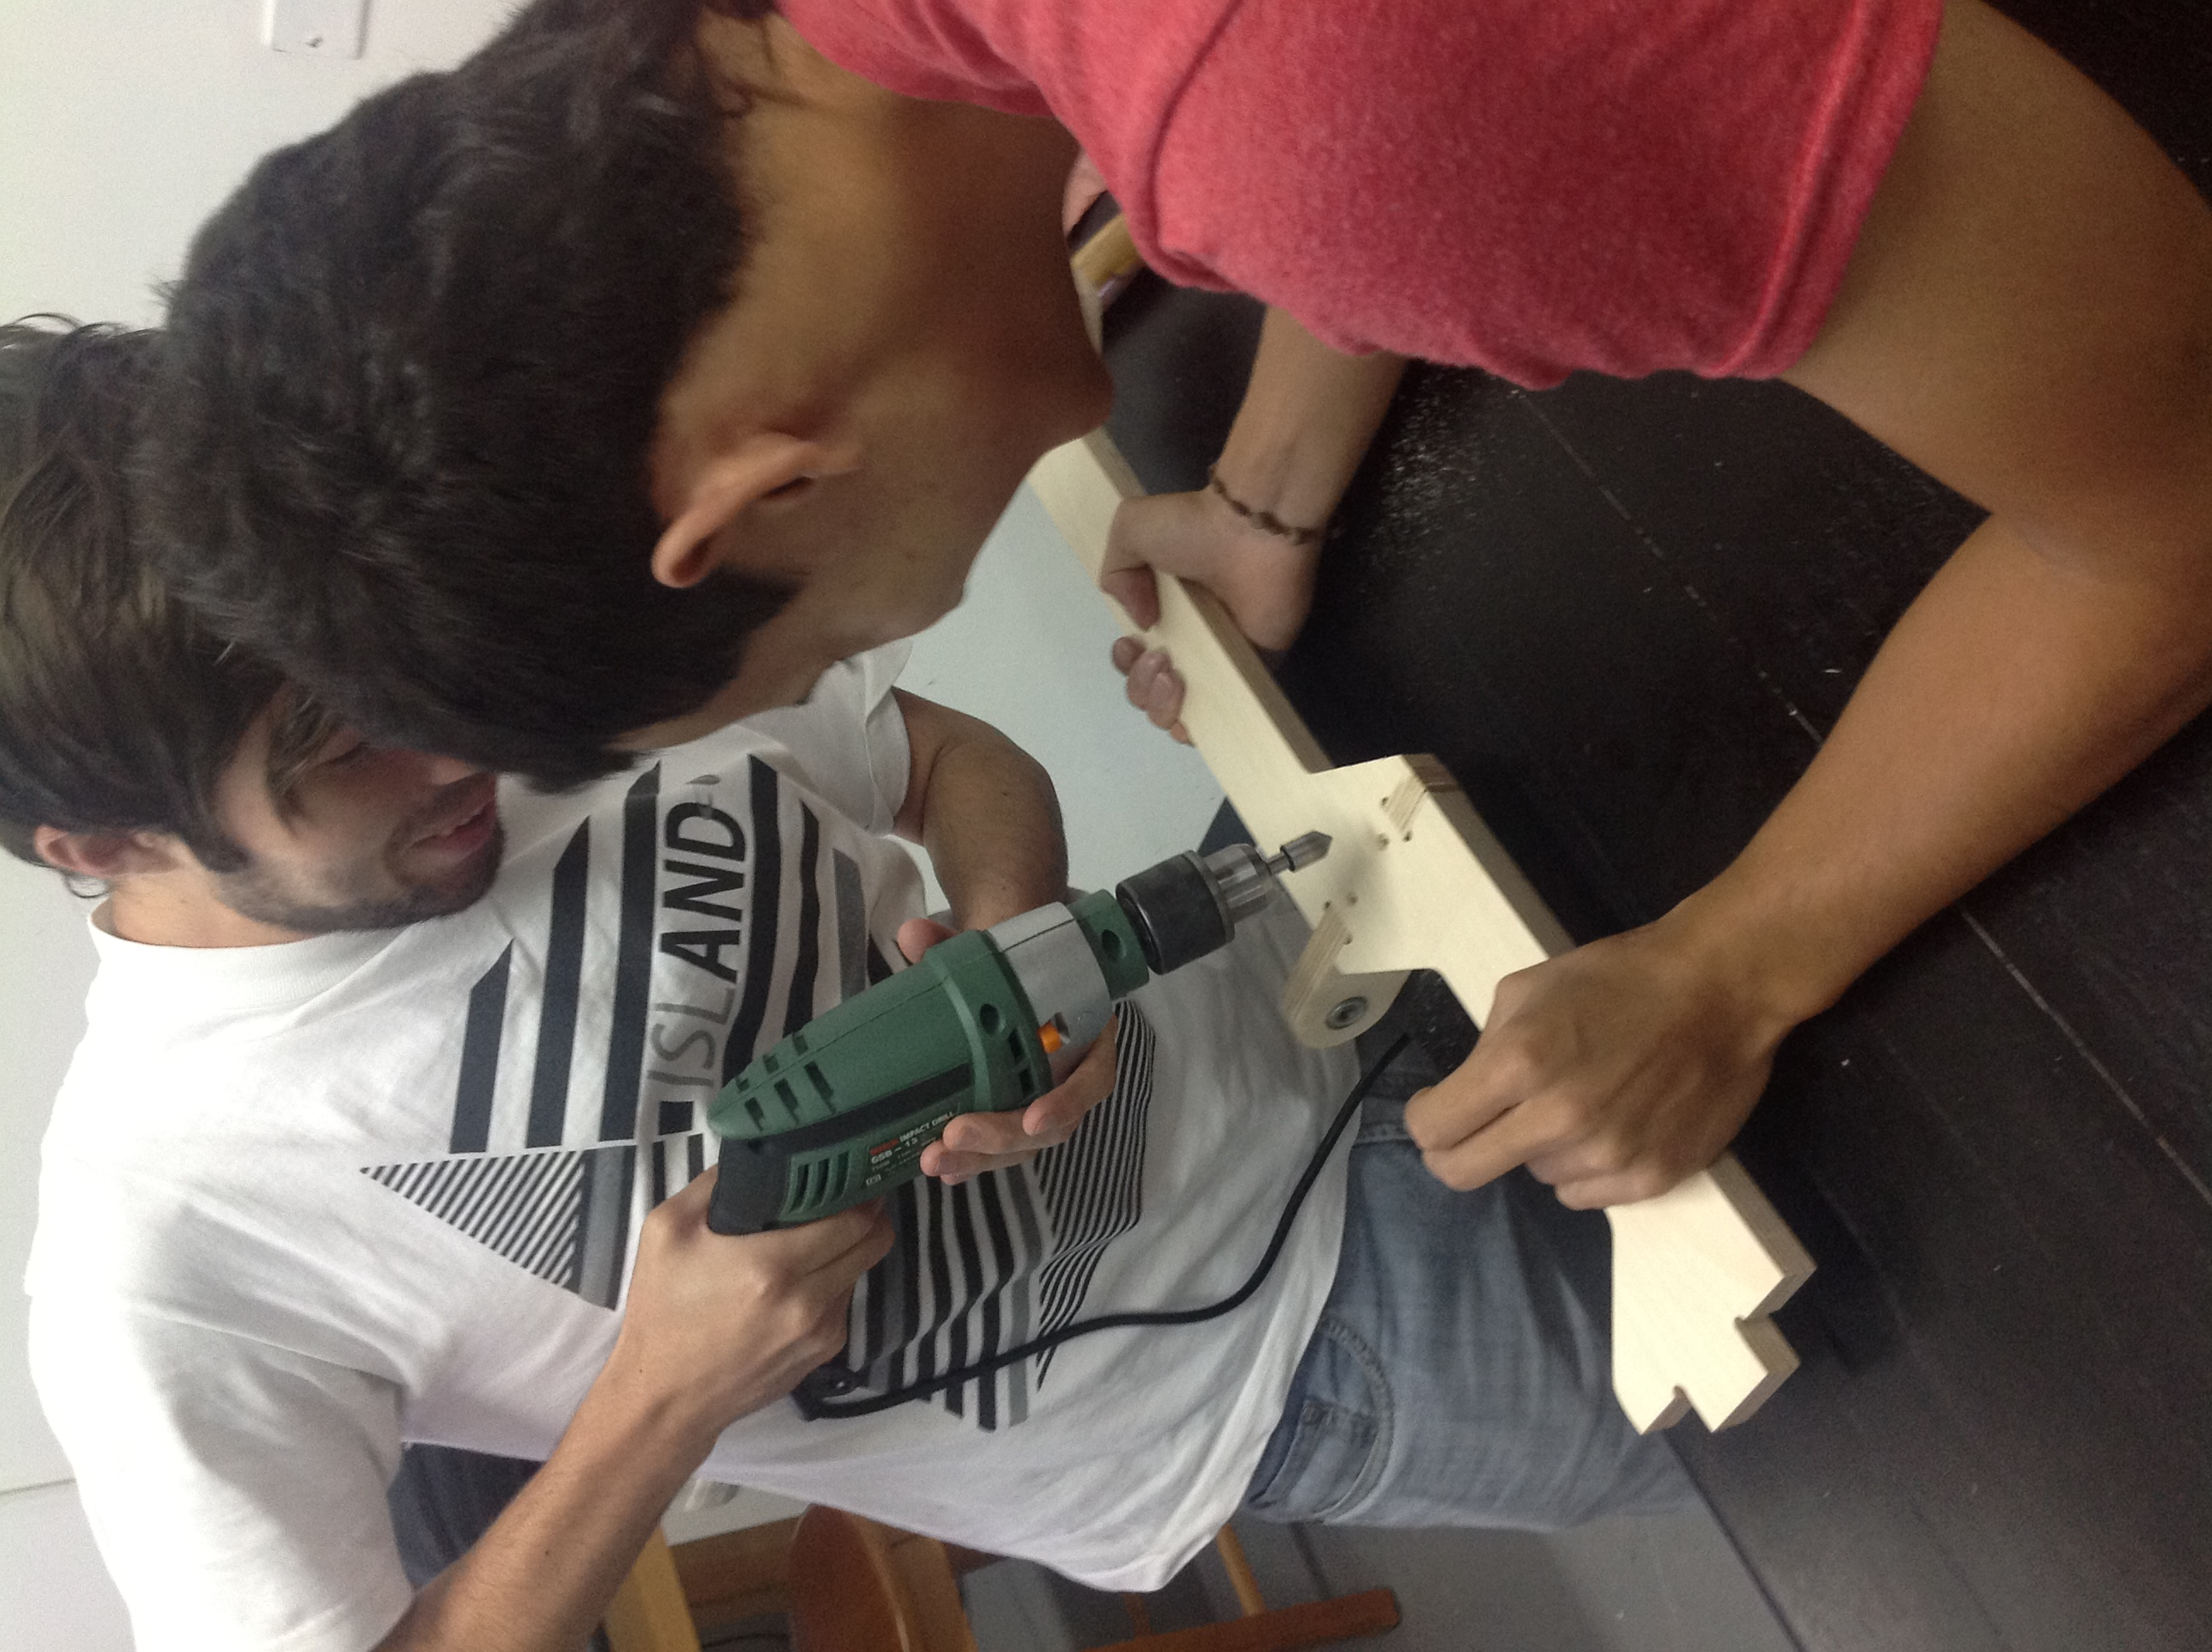
\includegraphics[width=2.5in]{escaner-estudiantes_trabajando}
% where an .eps filename suffix will be assumed under latex, 
% and a .pdf suffix will be assumed for pdflatex; or what has been declared
% via \DeclareGraphicsExtensions.
\caption{Estudiantes trabajando en el ensamblaje del escaner.}
\label{escaner}
\end{figure}
%%Ayuda: Falta una tile en escáner pero tex croma cuando la agrego

% Note that IEEE typically puts floats only at the top, even when this
% results in a large percentage of a column being occupied by floats.



\section{Resultados}

%Resultados de análsis del año 2013
En el caso del primer objetivo un elemento fundamental para brindar el apoyo
efectivo a los cursos de la carrera tiene relación directa con el
establecimiento de un espacio físico para trabajar y con materiales
computacionales necesarias, ambos elementos no fueron posibles de conseguir en
este periodo de tiempo. 



Al finalizar el 2014: 2 borradores de propuestas de investigación para ser
presentadas a las VIE en la ronda del 2015, dado que la presentación de las
propuestas es en mayo todavía se dispone de bastante tiempo para refinarlas. 

2013-2014:Exposición a público general: días de la libertad de software
(Alajuela, limón)[nota al pie: explicar qué es el SFD, que fue apoyado por la
municipalidad de Alajuela y que tuvo amplia difusión en medios de prensa],
semana Interunivesitaria (buses), día de la sede. 

%%tomar en cuenta la asociación con los objetivos del laboratorio. 
La proyección a la comunidad se pudo concretar por medio de la participaron del
proyecto “Escáner” en la actividad del Día de la Libertad de Software llevada a
cabo en la misma Sede Interuniversitaria durante el mes de setiembre del 2013 y
2014.

Al finalizar 2014: Espacio físico destinado para trabajar y materiales
suficientes para cumplir con el propósito de experimentar con tecnologías.  

% An example of a floating figure using the graphicx package.
% Note that \label must occur AFTER (or within) \caption.
% For figures, \caption should occur after the \includegraphics.
\begin{figure}[!t]
\centering
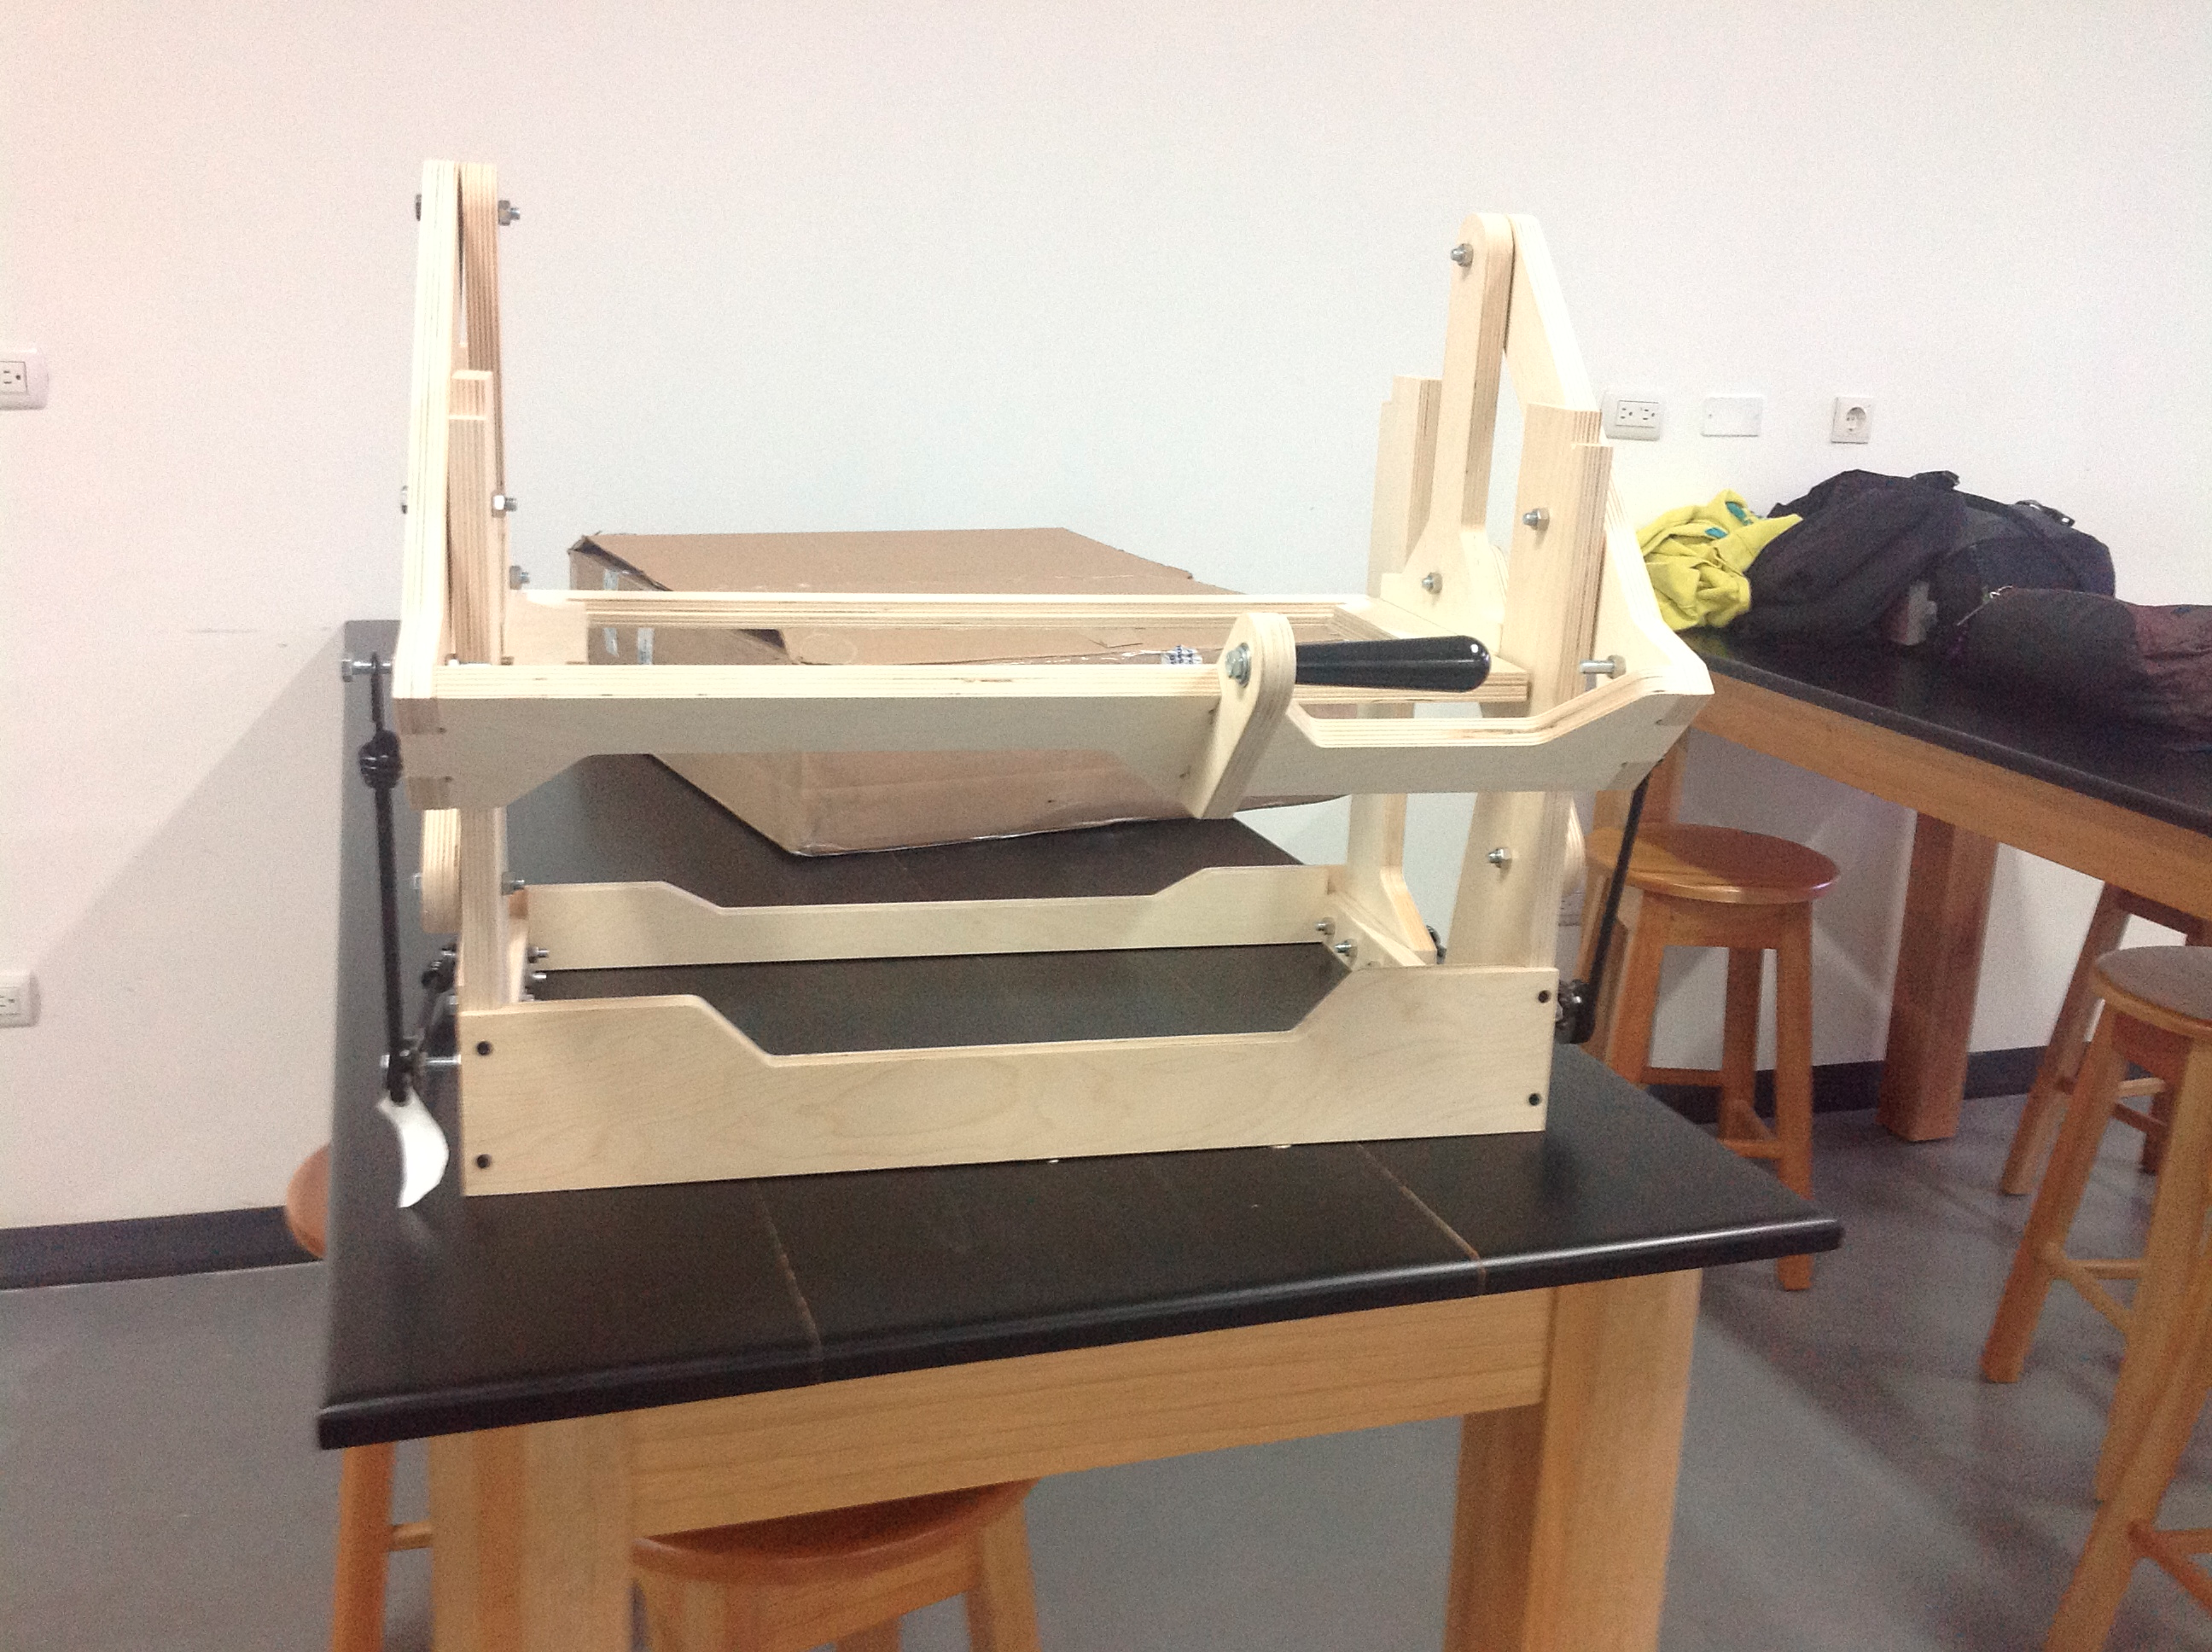
\includegraphics[width=2.5in]{escaner-mitad_ensamblaje}
% where an .eps filename suffix will be assumed under latex, 
% and a .pdf suffix will be assumed for pdflatex; or what has been declared
% via \DeclareGraphicsExtensions.
\caption{El escaner a mitad del ensamblaje.}
\label{escaner}
\end{figure}
%%Ayuda: Falta una tile en escáner pero tex croma cuando la agrego

% Note that IEEE typically puts floats only at the top, even when this
% results in a large percentage of a column being occupied by floats.




\section{Conclusiones y trabajo futuro}

Al finalizar el 2014 nos parece que el LabExp ha ofrecido a los estudiantes involucrados un espacio donde:

\begin{itemize}
    \item se enfrentaron a problemas técnicos novedosos para ellos, 
    \item profundiza en conceptos de Ingeniería de Software
    \item Software libre -> ver código
    \item ambientes de programación grupales (habilidades sociales de programación)
    \item un proceso de investigación con los estudiantes.
\end{itemize}

Los aspectos que justificaron la creación del Laboratorio experimental se
cumplieron completamente. El trabajo desarrollado en el Laboratorio Experimetal
se convirtió en el único espacio de investigación y extensión de la carrera de
Ing. en Computación en la SIU evidenciado en el proceso de acreditación al que
se sometió la carrera a finales del 2014. La participación de los estudiantes en
distintas actividad orientadas a la comunidad, presentando los proyectos en los
que trabajaron permitieron visibilizar la presencia del Tecnológico de Costa
Rica entre la comunidad Alajuelense cercana a la Sede Interuniversitaria. 

%%agregar acá el tema de la generación de propuesta como parte del objetivo 2 del laboratorio. 

Trabajo futuro: consolidación de los proyectos y esquemas de trabajo, mejorar la
divulgación de los proyectos (principalmente en el ámbito académico), establecer
mecanismos para incorporar nuevos miembros (profesores y estudiantes),
establecer vínculos con otras carreras de la SIU para trabajar en conjunto. 


% references section

% can use a bibliography generated by BibTeX as a .bbl file
% BibTeX documentation can be easily obtained at:
% http://www.ctan.org/tex-archive/biblio/bibtex/contrib/doc/
% The IEEEtran BibTeX style support page is at:
% http://www.michaelshell.org/tex/ieeetran/bibtex/
\bibliographystyle{IEEEtran}
% argument is your BibTeX string definitions and bibliography database(s)
\bibliography{labexp1.bib}
%
% <OR> manually copy in the resultant .bbl file
% set second argument of \begin to the number of references
% (used to reserve space for the reference number labels box)
%\begin{thebibliography}{3}


%\end{thebibliography}




% that's all folks
\end{document}



%\subsection{Subsection Heading Here}
%Subsection text here.


%\subsubsection{Subsubsection Heading Here}
%Subsubsection text here.


% An example of a floating figure using the graphicx package.
% Note that \label must occur AFTER (or within) \caption.
% For figures, \caption should occur after the \includegraphics.
% Note that IEEEtran v1.7 and later has special internal code that
% is designed to preserve the operation of \label within \caption
% even when the captionsoff option is in effect. However, because
% of issues like this, it may be the safest practice to put all your
% \label just after \caption rather than within \caption{}.
%
% Reminder: the "draftcls" or "draftclsnofoot", not "draft", class
% option should be used if it is desired that the figures are to be
% displayed while in draft mode.
%
%\begin{figure}[!t]
%\centering
%\includegraphics[width=2.5in]{myfigure}
% where an .eps filename suffix will be assumed under latex, 
% and a .pdf suffix will be assumed for pdflatex; or what has been declared
% via \DeclareGraphicsExtensions.
%\caption{Simulation Results}
%\label{fig_sim}
%\end{figure}

% Note that IEEE typically puts floats only at the top, even when this
% results in a large percentage of a column being occupied by floats.


% An example of a double column floating figure using two subfigures.
% (The subfig.sty package must be loaded for this to work.)
% The subfigure \label commands are set within each subfloat command, the
% \label for the overall figure must come after \caption.
% \hfil must be used as a separator to get equal spacing.
% The subfigure.sty package works much the same way, except \subfigure is
% used instead of \subfloat.
%
%\begin{figure*}[!t]
%\centerline{\subfloat[Case I]\includegraphics[width=2.5in]{subfigcase1}%
%\label{fig_first_case}}
%\hfil
%\subfloat[Case II]{\includegraphics[width=2.5in]{subfigcase2}%
%\label{fig_second_case}}}
%\caption{Simulation results}
%\label{fig_sim}
%\end{figure*}
%
% Note that often IEEE papers with subfigures do not employ subfigure
% captions (using the optional argument to \subfloat), but instead will
% reference/describe all of them (a), (b), etc., within the main caption.


% An example of a floating table. Note that, for IEEE style tables, the 
% \caption command should come BEFORE the table. Table text will default to
% \footnotesize as IEEE normally uses this smaller font for tables.
% The \label must come after \caption as always.
%
%\begin{table}[!t]
%% increase table row spacing, adjust to taste
%\renewcommand{\arraystretch}{1.3}
% if using array.sty, it might be a good idea to tweak the value of
% \extrarowheight as needed to properly center the text within the cells
%\caption{An Example of a Table}
%\label{table_example}
%\centering
%% Some packages, such as MDW tools, offer better commands for making tables
%% than the plain LaTeX2e tabular which is used here.
%\begin{tabular}{|c||c|}
%\hline
%One & Two\\
%\hline
%Three & Four\\
%\hline
%\end{tabular}
%\end{table}


% Note that IEEE does not put floats in the very first column - or typically
% anywhere on the first page for that matter. Also, in-text middle ("here")
% positioning is not used. Most IEEE journals/conferences use top floats
% exclusively. Note that, LaTeX2e, unlike IEEE journals/conferences, places
% footnotes above bottom floats. This can be corrected via the \fnbelowfloat
% command of the stfloats package.


% trigger a \newpage just before the given reference
% number - used to balance the columns on the last page
% adjust value as needed - may need to be readjusted if
% the document is modified later
%\IEEEtriggeratref{8}
% The "triggered" command can be changed if desired:
%\IEEEtriggercmd{\enlargethispage{-5in}}
